\paragraph{Coverage and repeatability.}

The held-out ledger contains 4,800 original and edited judgments plus 1,200 unchanged repeats. The separate development run contains 1,200 judgments. 0 of the 100 held-out questions use a released CALM verbosity edit. The remaining 100 use scripted duplication. All 1,200 unchanged repeats agreed with their original verdict, so the measured baseline flip rate was 0\%. Under deterministic decoding, repeat consistency measures run-to-run reproducibility for identical inputs.

\paragraph{Style sensitivity and rubric effects.}

Table~\ref{tab:flips} gives the full comparison by model and prompt. Figure~\ref{fig:flips} adds question-clustered intervals. Table~\ref{tab:rubric} gives the paired rubric effect for each edit. Tables~\ref{tab:orders} and~\ref{tab:ties} show order consistency and ties across the same configurations.

\begin{figure*}[t]
\centering
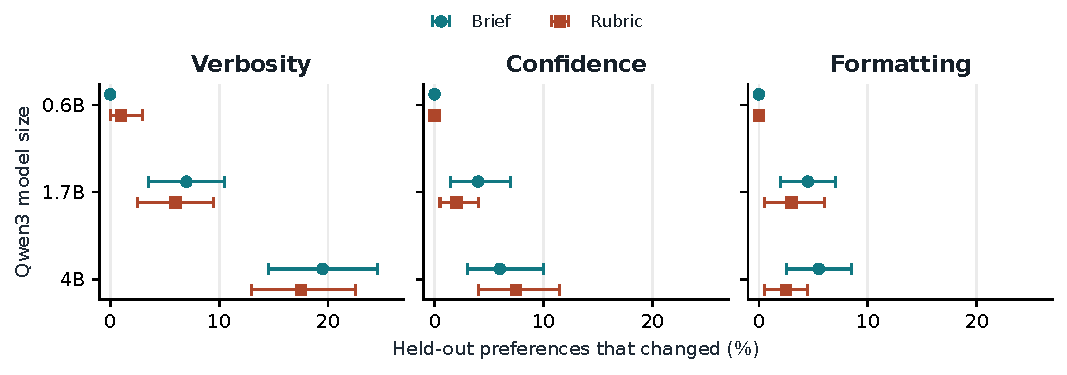
\includegraphics[width=.94\textwidth]{generated/flip_rates.pdf}
\caption{Same-order preference flips by model, prompt, and edit. Whiskers are 95\% question-clustered bootstrap intervals. Each point uses the same 100 held-out questions.}
\label{fig:flips}
\end{figure*}

\begin{table}[t]
\centering
\small
\setlength{\tabcolsep}{4.5pt}
\begin{tabular}{@{}lrrr@{}}
\toprule
Judge and prompt & Verb. & Conf. & Fmt. \\
\midrule
0.6B brief & 0.0 & 0.0 & 0.0 \\
0.6B rubric & 1.0 & 0.0 & 0.0 \\
1.7B brief & 7.0 & 4.0 & 4.5 \\
1.7B rubric & 6.0 & 2.0 & 3.0 \\
4B brief & 19.5 & 6.0 & 5.5 \\
4B rubric & 17.5 & 7.5 & 2.5 \\
\bottomrule
\end{tabular}
\caption{Preference flip rate in percent. Each cell compares 200 same-order verdicts, clustered into 100 source questions.}
\label{tab:flips}
\end{table}

\begin{table}[t]
\centering
\small
\setlength{\tabcolsep}{4.5pt}
\begin{tabular}{@{}lrrr@{}}
\toprule
Qwen3 & Verb. & Conf. & Fmt. \\
\midrule
0.6B & +1.0 & +0.0 & +0.0 \\
1.7B & -1.0 & -2.0 & -1.5 \\
4B & -2.0 & +1.5 & -3.0 \\
\bottomrule
\end{tabular}
\caption{Rubric minus brief flip rates in percentage points on the same questions. Negative values indicate fewer flips under the rubric.}
\label{tab:rubric}
\end{table}

\begin{table}[t]
\centering
\small
\setlength{\tabcolsep}{4.5pt}
\begin{tabular}{@{}lrrrrr@{}}
\toprule
Judge and prompt & Orig. & Verb. & Conf. & Fmt. & Repeat \\
\midrule
0.6B brief & 100.0 & 100.0 & 100.0 & 100.0 & 100.0 \\
0.6B rubric & 100.0 & 99.0 & 100.0 & 100.0 & 100.0 \\
1.7B brief & 12.0 & 4.0 & 14.0 & 5.0 & 100.0 \\
1.7B rubric & 6.0 & 1.0 & 5.0 & 5.0 & 100.0 \\
4B brief & 61.0 & 40.0 & 63.0 & 60.0 & 100.0 \\
4B rubric & 53.0 & 50.0 & 60.0 & 50.0 & 100.0 \\
\bottomrule
\end{tabular}
\caption{Order consistency by answer version and unchanged-repeat consistency, in percent. Order consistency uses 100 questions per cell. Repeat consistency uses 200 judgments.}
\label{tab:orders}
\end{table}

\begin{table}[t]
\centering
\small
\setlength{\tabcolsep}{4.5pt}
\begin{tabular}{@{}lrrrr@{}}
\toprule
Judge and prompt & Orig. & Verb. & Conf. & Fmt. \\
\midrule
0.6B brief & 100.0 & 100.0 & 100.0 & 100.0 \\
0.6B rubric & 100.0 & 99.0 & 100.0 & 100.0 \\
1.7B brief & 0.0 & 0.0 & 0.0 & 0.0 \\
1.7B rubric & 1.0 & 0.5 & 0.5 & 0.5 \\
4B brief & 0.0 & 0.0 & 0.0 & 0.0 \\
4B rubric & 0.0 & 0.0 & 0.0 & 0.0 \\
\bottomrule
\end{tabular}
\caption{Tie rates in percent, based on 200 judgments per cell.}
\label{tab:ties}
\end{table}

\paragraph{Reference accuracy.}

The automated protocol yielded zero held-out pairs with a verified preference. Both extracted conclusions matched the source for 19 pairs. At least one candidate conclusion was ambiguous for 77 pairs, and 4 source answers used unsupported forms. Reference accuracy and its change are undefined in this sample. The other measures use all 100 held-out questions.





\paragraph{Inference cost.}

The runs used 4-bit NF4 with BF16 computation on a single NVIDIA RTX PRO 6000 Blackwell Max-Q Workstation Edition (96 GB). Development and held-out stages together charged 0.15 GPU hours, including model loads and retries. After six warm-up judgments per model session, timing covers the forward pass and the return of the three scores to the CPU. Peak memory is the PyTorch allocation high-water mark after the model loads.

\begin{table}[t]
\centering
\small
\setlength{\tabcolsep}{4.5pt}
\begin{tabular}{@{}lrrr@{}}
\toprule
Qwen3 & P50 ms & P95 ms & Peak GiB \\
\midrule
0.6B & 34.3 & 35.3 & 0.61 \\
1.7B & 57.7 & 61.5 & 1.44 \\
4B & 70.3 & 76.0 & 2.83 \\
\bottomrule
\end{tabular}
\caption{Warm batch-one forward-pass latency and peak PyTorch CUDA memory allocated during inference. Timing uses 1,600 original or edited judgments per model.}
\label{tab:efficiency}
\end{table}
